
\documentclass[11pt]{article}
\usepackage[a4paper,margin=1in]{geometry}
\usepackage{amsmath,amssymb}
\usepackage{graphicx}
\usepackage[dvipsnames]{xcolor}
\usepackage{hyperref}
\usepackage{enumitem}
\usepackage{tabularx}
\usepackage{longtable}
\usepackage{booktabs}
\usepackage[most]{tcolorbox}
\usepackage{titlesec}
\usepackage{xurl}
\usepackage{fancyhdr}
\usepackage{setspace}
\usepackage{tikz}
\usetikzlibrary{positioning,arrows.meta}
\usepackage[T1]{fontenc}
\usepackage{lmodern}
\setlength{\parindent}{0pt}
\setlength{\parskip}{8pt}
\setlength{\headheight}{14pt}
\setstretch{1.12}
\setlist[itemize]{leftmargin=1.5em, nosep}
\setlist[enumerate]{leftmargin=1.5em, nosep}
\providecommand{\tightlist}{\setlength{\itemsep}{0pt}\setlength{\parskip}{0pt}}
\hypersetup{colorlinks=true,linkcolor=MidnightBlue,urlcolor=MidnightBlue}
\pagestyle{fancy}
\fancyhf{}
\rhead{\thepage}
\renewcommand{\headrulewidth}{0pt}
\renewcommand{\footrulewidth}{0pt}
\titleformat{\section}{\Large\bfseries\color{MidnightBlue}}{\thesection}{0.6em}{}
\titleformat{\subsection}{\bfseries}{}{0em}{}


\begin{document}

\begin{center}\LARGE\bfseries Planning with Uncertainty\end{center}

\begin{center}\large Block 4 Day 4\end{center}

\begin{tcolorbox}[colback=MidnightBlue!4,colframe=MidnightBlue,title={Session Overview},fonttitle=\bfseries,breakable]
\textbf{Session objective:} Move from utility and decision networks to sequential planning with Markov decision processes and the limits of full observability.

\textbf{Timing target (min):} 71

\textbf{Topic anchors:} utility; expected utility; decision network; markov decision process; value iteration; policy iteration

\textbf{Padlet board:} \url{https://padlet.com/qmul/b4-d4-4yoefwupfn46p8ph}
\end{tcolorbox}

\section*{Exercises}

\begin{tcolorbox}[colback=white,colframe=MidnightBlue,title={Q1 Starter Classification},fonttitle=\bfseries,breakable]
\begin{center}
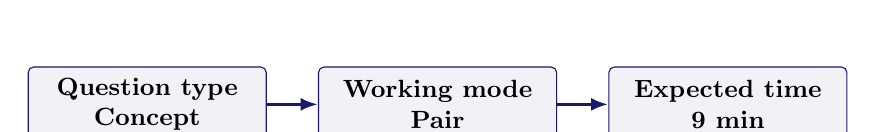
\begin{tikzpicture}[
node distance=0.65cm,
box/.style={draw=MidnightBlue, rounded corners=2pt, minimum height=0.95cm, align=center, font=\small\bfseries, fill=MidnightBlue!6, text width=0.23\linewidth},
arrow/.style={-{Latex[length=2.2mm]}, very thick, MidnightBlue}
]
\node[box] (type) {Question type\\Concept};
\node[box, right=of type] (mode) {Working mode\\Pair};
\node[box, right=of mode] (time) {Expected time\\9 min};
\draw[arrow] (type) -- (mode);
\draw[arrow] (mode) -- (time);
\end{tikzpicture}
\end{center}

{\large\bfseries\color{MidnightBlue} Prompt}\par\medskip
In an emergency drone-routing problem, classify these items as feature, preference, or utility term: battery level, wind speed, avoid school zone, short travel time, crash penalty, and patient arrival bonus. Then explain why mixing these categories causes planning mistakes.

{\large\bfseries\color{MidnightBlue} Task details}\par\medskip
\begin{itemize}\item \textbf{Type:} concept
\item \textbf{Mode:} pair
\item \textbf{Time:} 9 min
\item \textbf{Deliverable:} concept table
\item \textbf{Assessment focus:} separate features, preferences, and numeric utility terms
\item \textbf{Expected length:} 6 labels + 1 explanation\end{itemize}

{\large\bfseries\color{MidnightBlue} How to submit}\par\medskip
Post one pair Padlet comment as a six-row table plus one short explanation.

{\large\bfseries\color{MidnightBlue} Discussion in class}\par\medskip
Which item is easiest to classify wrongly?

{\large\bfseries\color{MidnightBlue} Why this helps}\par\medskip
Useful for questions that ask students to separate the world description from the planner's objective.

{\large\bfseries\color{MidnightBlue} References}\par\medskip
\begin{itemize}\item Russell \& Norvig (2021) AIMA 4e, Ch.16-17
\item Poole \& Mackworth (2023) 3e, Ch.12, pp.517-582\end{itemize}
\end{tcolorbox}

\begin{tcolorbox}[colback=white,colframe=MidnightBlue,title={Q2 Structured Problem},fonttitle=\bfseries,breakable]
\begin{center}
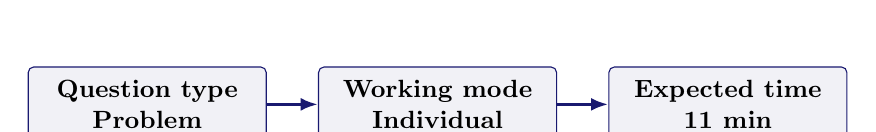
\begin{tikzpicture}[
node distance=0.65cm,
box/.style={draw=MidnightBlue, rounded corners=2pt, minimum height=0.95cm, align=center, font=\small\bfseries, fill=MidnightBlue!6, text width=0.23\linewidth},
arrow/.style={-{Latex[length=2.2mm]}, very thick, MidnightBlue}
]
\node[box] (type) {Question type\\Problem};
\node[box, right=of type] (mode) {Working mode\\Individual};
\node[box, right=of mode] (time) {Expected time\\11 min};
\draw[arrow] (type) -- (mode);
\draw[arrow] (mode) -- (time);
\end{tikzpicture}
\end{center}

{\large\bfseries\color{MidnightBlue} Prompt}\par\medskip
A delivery agent has two route choices. Fast route: with probability 0.6 it arrives on time for utility +12, and with probability 0.4 it suffers severe delay for utility -10. Safe route: with probability 0.85 it arrives on time for utility +8, and with probability 0.15 it suffers mild delay for utility +1. Compute expected utility for both actions and choose the better one.

\begin{tcolorbox}[colback=ForestGreen!5,colframe=ForestGreen,title={Formula reminder},fonttitle=\bfseries,breakable]
\[
EU(a)=\sum_{s} P(s \mid e)\,U(s,a)
\]
\textbf{Use this when the task asks you to compare actions under uncertainty.}
\end{tcolorbox}

{\large\bfseries\color{MidnightBlue} Task details}\par\medskip
\begin{itemize}\item \textbf{Type:} problem
\item \textbf{Mode:} individual
\item \textbf{Time:} 11 min
\item \textbf{Deliverable:} expected utility computation
\item \textbf{Assessment focus:} compute expected utility and choose the better action
\item \textbf{Expected length:} 4 calculation lines\end{itemize}

{\large\bfseries\color{MidnightBlue} How to submit}\par\medskip
Post your own Padlet comment showing both expected-utility calculations and the chosen action.

{\large\bfseries\color{MidnightBlue} Discussion in class}\par\medskip
Why can the route with the larger best-case reward still be the worse decision?

{\large\bfseries\color{MidnightBlue} Why this helps}\par\medskip
Direct practice for expected-utility calculations without duplicating the exam numbers.

{\large\bfseries\color{MidnightBlue} References}\par\medskip
\begin{itemize}\item Russell \& Norvig (2021) AIMA 4e, Ch.16-17
\item Poole \& Mackworth (2023) 3e, Ch.12, pp.517-582\end{itemize}
\end{tcolorbox}

\begin{tcolorbox}[colback=white,colframe=MidnightBlue,title={Q3 Structured Problem},fonttitle=\bfseries,breakable]
\begin{center}
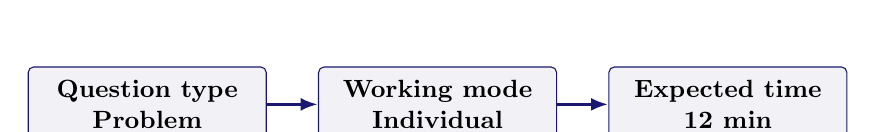
\begin{tikzpicture}[
node distance=0.65cm,
box/.style={draw=MidnightBlue, rounded corners=2pt, minimum height=0.95cm, align=center, font=\small\bfseries, fill=MidnightBlue!6, text width=0.23\linewidth},
arrow/.style={-{Latex[length=2.2mm]}, very thick, MidnightBlue}
]
\node[box] (type) {Question type\\Problem};
\node[box, right=of type] (mode) {Working mode\\Individual};
\node[box, right=of mode] (time) {Expected time\\12 min};
\draw[arrow] (type) -- (mode);
\draw[arrow] (mode) -- (time);
\end{tikzpicture}
\end{center}

{\large\bfseries\color{MidnightBlue} Prompt}\par\medskip
For each scenario, choose the most suitable planning model and explain why: (1) a one-off hiring decision with uncertain outcomes, (2) a warehouse robot making repeated fully observed navigation choices, and (3) a rescue robot acting repeatedly when the true hazard level is only partly visible. Choose from decision network, Markov decision process (MDP), or partially observable Markov decision process (POMDP).

{\large\bfseries\color{MidnightBlue} Task details}\par\medskip
\begin{itemize}\item \textbf{Type:} problem
\item \textbf{Mode:} individual
\item \textbf{Time:} 12 min
\item \textbf{Deliverable:} model-choice explanation
\item \textbf{Assessment focus:} choose between a decision network, a Markov decision process, and a POMDP-style view
\item \textbf{Expected length:} 3 short cases\end{itemize}

{\large\bfseries\color{MidnightBlue} How to submit}\par\medskip
Post your own Padlet comment with three choices and one short reason each.

{\large\bfseries\color{MidnightBlue} Discussion in class}\par\medskip
Which feature forces you away from an ordinary MDP?

{\large\bfseries\color{MidnightBlue} Why this helps}\par\medskip
Useful for model-selection questions that test when partial observability changes the planning model.

{\large\bfseries\color{MidnightBlue} References}\par\medskip
\begin{itemize}\item Russell \& Norvig (2021) AIMA 4e, Ch.16-17
\item Poole \& Mackworth (2023) 3e, Ch.12, pp.517-582\end{itemize}
\end{tcolorbox}

\begin{tcolorbox}[colback=white,colframe=MidnightBlue,title={Q4 Collaborative Mini-Case},fonttitle=\bfseries,breakable]
\begin{center}
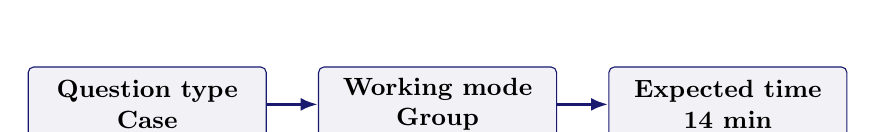
\begin{tikzpicture}[
node distance=0.65cm,
box/.style={draw=MidnightBlue, rounded corners=2pt, minimum height=0.95cm, align=center, font=\small\bfseries, fill=MidnightBlue!6, text width=0.23\linewidth},
arrow/.style={-{Latex[length=2.2mm]}, very thick, MidnightBlue}
]
\node[box] (type) {Question type\\Case};
\node[box, right=of type] (mode) {Working mode\\Group};
\node[box, right=of mode] (time) {Expected time\\14 min};
\draw[arrow] (type) -- (mode);
\draw[arrow] (mode) -- (time);
\end{tikzpicture}
\end{center}

{\large\bfseries\color{MidnightBlue} Prompt}\par\medskip
Design a hospital-delivery robot planning setup that shows the difference between a one-off choice and a sequential choice. Include state, action, uncertainty, utility, and one reason the system might later need a belief-based view rather than a plain MDP.

{\large\bfseries\color{MidnightBlue} Task details}\par\medskip
\begin{itemize}\item \textbf{Type:} case
\item \textbf{Mode:} group
\item \textbf{Time:} 14 min
\item \textbf{Deliverable:} sequential planning sketch
\item \textbf{Assessment focus:} design a small planning setup that clearly becomes sequential
\item \textbf{Expected length:} 5 bullets + 1 note\end{itemize}

{\large\bfseries\color{MidnightBlue} How to submit}\par\medskip
Post one group Padlet comment with the planning setup and one note on where uncertainty changes the choice.

{\large\bfseries\color{MidnightBlue} Discussion in class}\par\medskip
Which part of your design makes the problem sequential instead of one-shot?

{\large\bfseries\color{MidnightBlue} Why this helps}\par\medskip
Supports case questions on moving from simple decision analysis to sequential planning.

{\large\bfseries\color{MidnightBlue} References}\par\medskip
\begin{itemize}\item Russell \& Norvig (2021) AIMA 4e, Ch.16-17
\item Poole \& Mackworth (2023) 3e, Ch.12, pp.517-582\end{itemize}
\end{tcolorbox}

\begin{tcolorbox}[colback=white,colframe=MidnightBlue,title={Q5 Exam-Style Constructed Response},fonttitle=\bfseries,breakable]
\begin{center}
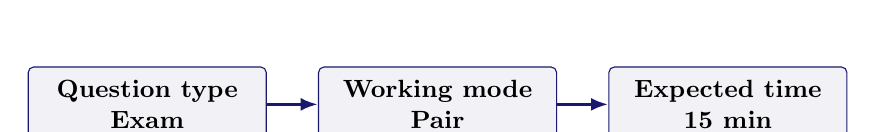
\begin{tikzpicture}[
node distance=0.65cm,
box/.style={draw=MidnightBlue, rounded corners=2pt, minimum height=0.95cm, align=center, font=\small\bfseries, fill=MidnightBlue!6, text width=0.23\linewidth},
arrow/.style={-{Latex[length=2.2mm]}, very thick, MidnightBlue}
]
\node[box] (type) {Question type\\Exam};
\node[box, right=of type] (mode) {Working mode\\Pair};
\node[box, right=of mode] (time) {Expected time\\15 min};
\draw[arrow] (type) -- (mode);
\draw[arrow] (mode) -- (time);
\end{tikzpicture}
\end{center}

{\large\bfseries\color{MidnightBlue} Prompt}\par\medskip
Explain the difference between planning in a Markov decision process with a known model and learning by reinforcement in the same environment. Then add one short note on why partial observability makes planning harder.

{\large\bfseries\color{MidnightBlue} Task details}\par\medskip
\begin{itemize}\item \textbf{Type:} exam
\item \textbf{Mode:} pair
\item \textbf{Time:} 15 min
\item \textbf{Deliverable:} written argument
\item \textbf{Assessment focus:} compare planning in a Markov decision process with learning by reinforcement
\item \textbf{Expected length:} 180-240 words\end{itemize}

{\large\bfseries\color{MidnightBlue} How to submit}\par\medskip
Post one pair Padlet comment with a clear comparison, one reason the known model matters, and one note on partial observability.

{\large\bfseries\color{MidnightBlue} Discussion in class}\par\medskip
Why is planning in an MDP not just ``reinforcement learning done more carefully''?

{\large\bfseries\color{MidnightBlue} Why this helps}\par\medskip
Strengthens comparison of planning and learning methods in a new setting.

{\large\bfseries\color{MidnightBlue} References}\par\medskip
\begin{itemize}\item Russell \& Norvig (2021) AIMA 4e, Ch.16-17
\item Poole \& Mackworth (2023) 3e, Ch.12, pp.517-582\end{itemize}
\end{tcolorbox}

\begin{tcolorbox}[colback=white,colframe=MidnightBlue,title={Q6 Stretch Extension},fonttitle=\bfseries,breakable]
\begin{center}
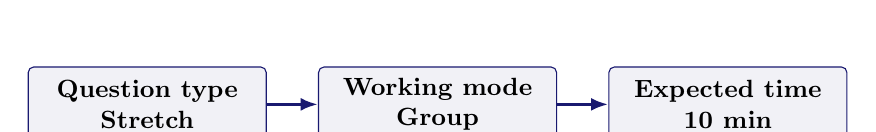
\begin{tikzpicture}[
node distance=0.65cm,
box/.style={draw=MidnightBlue, rounded corners=2pt, minimum height=0.95cm, align=center, font=\small\bfseries, fill=MidnightBlue!6, text width=0.23\linewidth},
arrow/.style={-{Latex[length=2.2mm]}, very thick, MidnightBlue}
]
\node[box] (type) {Question type\\Stretch};
\node[box, right=of type] (mode) {Working mode\\Group};
\node[box, right=of mode] (time) {Expected time\\10 min};
\draw[arrow] (type) -- (mode);
\draw[arrow] (mode) -- (time);
\end{tikzpicture}
\end{center}

{\large\bfseries\color{MidnightBlue} Prompt}\par\medskip
Build a short safety checklist for uncertain planning in a high-risk domain such as healthcare delivery, emergency response, or cybersecurity response.

{\large\bfseries\color{MidnightBlue} Task details}\par\medskip
\begin{itemize}\item \textbf{Type:} stretch
\item \textbf{Mode:} group
\item \textbf{Time:} 10 min
\item \textbf{Deliverable:} safety checklist
\item \textbf{Assessment focus:} turn uncertain planning into operational controls
\item \textbf{Expected length:} 4-5 checklist items\end{itemize}

{\large\bfseries\color{MidnightBlue} How to submit}\par\medskip
Post one group Padlet comment with four or five controls and say which one should be enforced first.

{\large\bfseries\color{MidnightBlue} Discussion in class}\par\medskip
Which safety check protects against the worst planning mistake?

{\large\bfseries\color{MidnightBlue} Why this helps}\par\medskip
Good extension for questions that ask students to move from planning theory to safe deployment.

{\large\bfseries\color{MidnightBlue} References}\par\medskip
\begin{itemize}\item Russell \& Norvig (2021) AIMA 4e, Ch.16-17
\item Poole \& Mackworth (2023) 3e, Ch.12, pp.517-582\end{itemize}
\end{tcolorbox}

\section*{Submission Instructions}

Use the seeded Padlet posts for Q1--Q6. Q2 and Q3 are individual. Q1 and Q5 are pair tasks. Q4 and Q6 should be one joint group comment. Start each comment with your names or group label.

\section*{Whole-Class Debrief Prompts}

\begin{itemize}
\tightlist
\item
  Which utility calculation changed the decision most?
\item
  What makes a planning problem sequential rather than one-off?
\item
  When does partial observability force you to change the planning model completely?
\end{itemize}

\section*{Exam Transfer Note (Day-Level)}

Maps to exam questions on utility, expected utility, decision networks, Markov decision processes, and planning under limited observability.

\end{document}
